\documentclass[a4paper]{article}

\usepackage[english]{babel}
\usepackage[utf8]{inputenc}
\usepackage{amsmath}
\usepackage{graphicx}

\title{Finding a Minimum-Weight Spanning Tree Using Gallager, Humblet and Spira's Algorithm}

\author{Jens de Waard \\ 4009215 \and Tim Wissel \\ 4xxxxxx}

\date{\today}

\begin{document}
\maketitle

\begin{abstract}
Enter a short summary here. What topic do you want to investigate and why? What experiment did you perform? What were your main results and conclusion?
\end{abstract}

\tableofcontents

\section{Introduction 5 lines to max 1/2 page}
\label{sec:introduction}

Explain the context of the experiment here. Why is condensed matter physics interesting or important?
Optional things you could talk about (but don't have to -- this is up to you): transistors, computers, Quantum computers, fundamental knowledge (e.g. the resistance quantum).

Briefly explain what methods you will use in the experiment, and what values you will extract from the data.

For this section and all following sections: If you refer to an equation, previous result or theory that is not regarded as common knowledge, then cite the source (article or book) where you found this. For example, you can cite the Nano 3 Lecture notes \cite{nano3}.

\section{Implementation Details}
\label{sec:implementation}

\section{Results}
\label{sec:results}

\begin{figure}
\centering
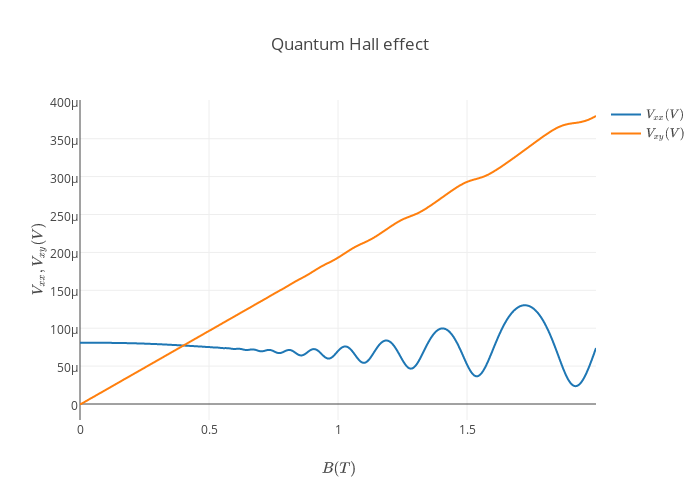
\includegraphics[width=1\textwidth]{raw_data.png}
\caption{\label{fig:data}Raw (unprocessed) data. Replace this figure with the one you've made, that shows the resistivity.}
\end{figure}

\section{Conclusion}
\label{sec:conclusion}

\begin{thebibliography}{9}
\bibitem{nano3}
  K. Grove-Rasmussen og Jesper Nygård,
  \emph{Kvantefænomener i Nanosystemer}.
  Niels Bohr Institute \& Nano-Science Center, Københavns Universitet

\end{thebibliography}
\end{document}
